\documentclass{beamer}
\special{landscape}

%\usetheme{Berlin}
\usetheme{Warsaw}

%\usecolortheme{seahorse}
%\usefonttheme[onlysmall]{structurebold}

\setbeamertemplate{headline}[split]
\setbeamertemplate{footline}[default]
\setbeamertemplate{footline}[miniframes theme]
%\logo{\includegraphics[scale=0.5]{image/logo4c.gif}}

\mode<presentation>
\usepackage[spanish]{babel}
\usepackage{beamerthemesplit}
\usepackage[utf8]{inputenc}
\usepackage{color}      % use if color is used in text
\usepackage{pslatex}
\usepackage{graphicx}
\usepackage{amssymb}



% Comandos en modo Verbatim
\usepackage{fancyvrb}


\title{Conceptos Básicos de Geoestadística}
\author{Eloy Adonis Colell\\Juan Uribe\\Pablo Chale}

\institute{Universidad Nacional de Luján}
\date{\includegraphics[clip,scale=0.4]{document/image/by-nc-nd.eps}\\ \today}


\AtBeginSection[]

\begin{document}

\begin{frame}
\titlepage
\end{frame}


%\begin{frame}[t]%,allowframebreaks]
%\frametitle{Proyectos}
%\tableofcontents
%\end{frame}



\section{Series Temporales}
\begin{frame}
\frametitle{Series Temporales}
\begin{figure}
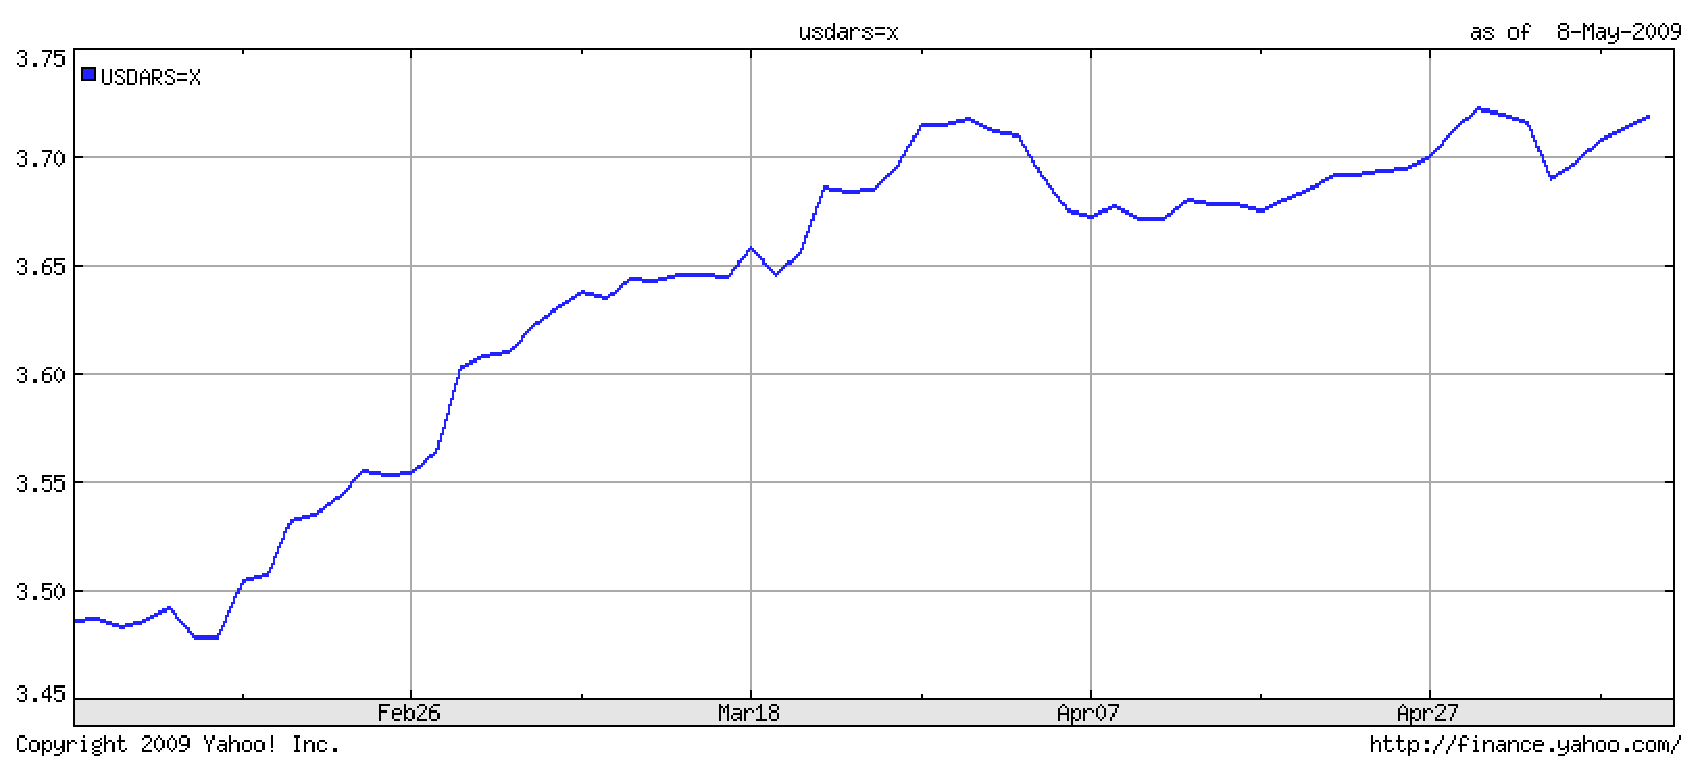
\includegraphics[scale=0.24]{image/usdars.eps}
\end{figure}
\begin{figure}
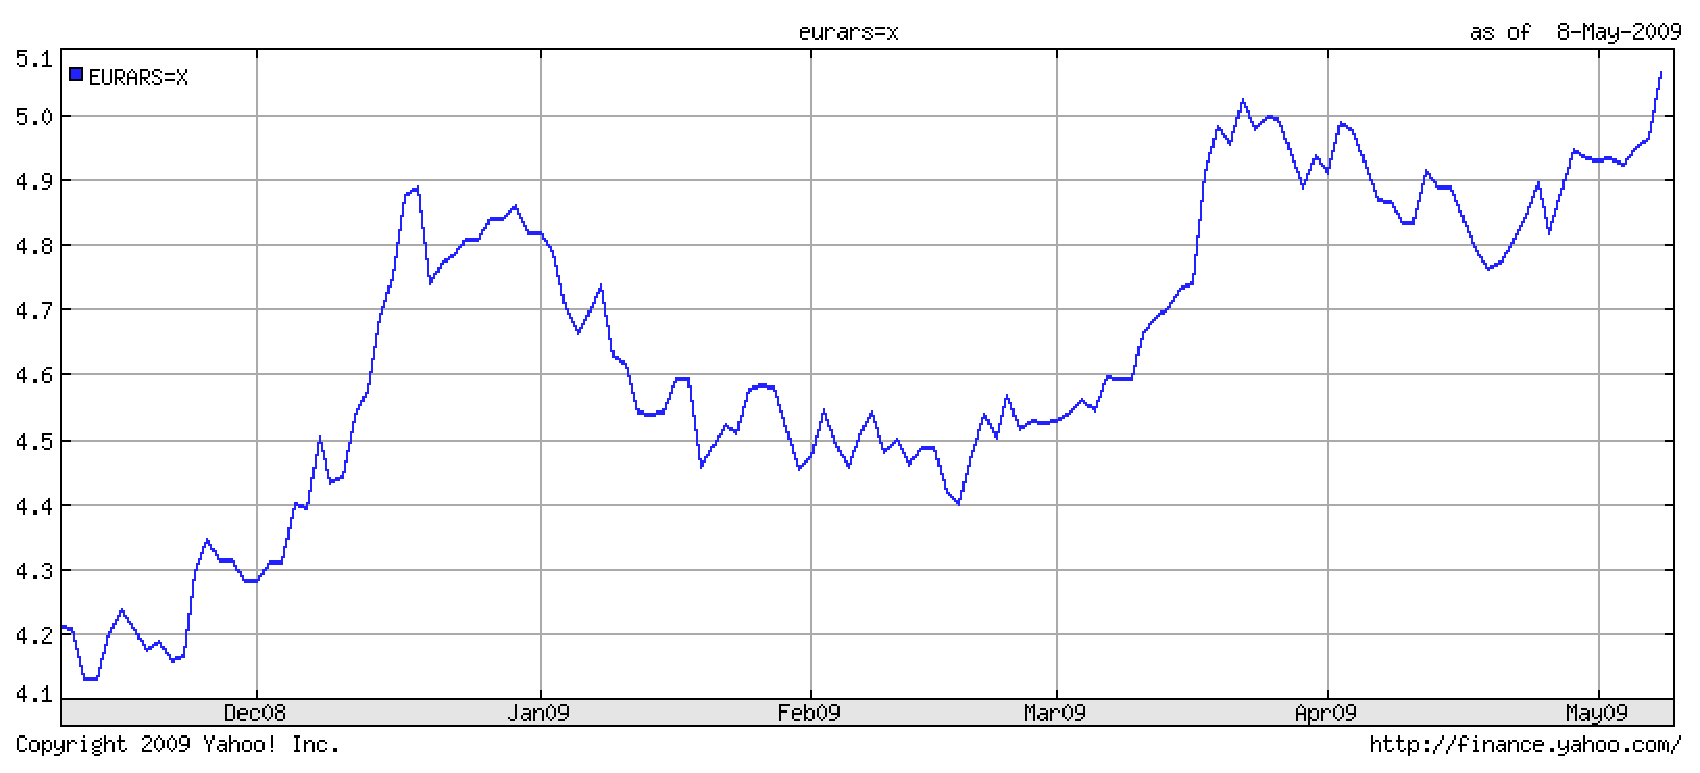
\includegraphics[scale=0.24]{image/eurars.eps}
\end{figure}
\end{frame}


\subsection{Enfoque Clásico}
\begin{frame}
\frametitle{Enfoque Clásico}
\begin{equation}
Z(t) = (T(t), E(t), C(t), R(t))
\end{equation}
\begin{itemize}
\item Tendencia (T)
\item Estacional (E)
\item Cíclica (C)
\item Residual (R)
\end{itemize}
\end{frame}

\begin{frame}
\frametitle{Tendencia (T)}
\begin{itemize}
\item Análisis gráfico
\item Alisado proporcional
\begin{itemize}
\item Medias móviles
\item Método analítico
\end{itemize}
\item Alisado exponencial
\end{itemize}
\end{frame}

\begin{frame}
\frametitle{Medias móviles}
\begin{figure}
\includegraphics[scale=0.5]{document/graph/g00008.eps}
\end{figure}
\begin{equation}
y_t^* = \displaystyle\frac{\displaystyle\sum_{i=-\frac{k-1}{2}}^{\frac{k-1}{2}}y_{t+i}}{k}
\end{equation}
\end{frame}

\begin{frame}
\frametitle{Método analítico - Lineal}
\begin{figure}
\includegraphics[scale=0.5]{document/graph/g00009.eps}
\end{figure}
\begin{equation}
y_t = y_t^* + R_t = a + bt + R_t
\end{equation}
\end{frame}

\begin{frame}
\frametitle{Método analítico - Polinomial}
\begin{figure}
\includegraphics[scale=0.5]{document/graph/g00010.eps}
\end{figure}
\begin{equation}
y_t = y_t^* + R_t = a + bt + ct^2 + R_t
\end{equation}
\end{frame}

\begin{frame}
\frametitle{Método analítico - Exponencial}
\begin{figure}
\includegraphics[scale=0.5]{document/graph/g00011.eps}
\end{figure}
\begin{equation}
y_t = y_t^* + R_t = a e^{bt} + R_t
\end{equation}
\end{frame}

\begin{frame}
\frametitle{Alisado exponencial}
La \emph{ponderación decrese} cuando nos alejamos del origen.
\begin{figure}
\includegraphics[scale=0.5]{document/graph/g00012.eps}
\end{figure}
\begin{equation}
y_t^* = \alpha y_t + (1-\alpha) y_{t-1}^*
\end{equation}
\end{frame}

\begin{frame}
\frametitle{Estacional (E)}
IGVE : Indices Generales de Variación Estacional
\begin{figure}
\includegraphics[scale=0.4]{document/graph/g00014.eps}
\includegraphics[scale=0.4]{document/graph/g00013.eps}
\end{figure}
\begin{equation}
y_t^* = y_t - (C_t + R_t); T_t \not \in y_t
\end{equation}
\end{frame}

\begin{frame}
\frametitle{Cíclica (C)}
Por medias móviles
\begin{figure}
\includegraphics[scale=0.5]{document/graph/g00015.eps}
\end{figure}
\end{frame}

\begin{frame}
\frametitle{Residual (R)}
\begin{itemize}
\item Valores aleatorios
\item No responde a un patrón de comportamiento
\item Sirve para verificar ciertos supuestos o hipótesis
\end{itemize}
\end{frame}


\subsection{Enfoque Causal}
\begin{frame}
\frametitle{Enfoque Causal}
\begin{equation}
\Delta y_t = y_t - y_{t-1}
\end{equation}
Tasas de variación
\begin{equation}
T(h,n) = T_h^n = \frac{\sum_{i=0}^{n-1}y_{t-i}}{\sum_{j=0}^{n-1}y_{t-h-j}}-1
\end{equation}
\begin{equation}
T(h,1) = T_h^1 = \frac{y_t}{y_{t-h}} -1 = \displaystyle\frac{y_t - y_{t-h}}{y_{t-h}} = \displaystyle\frac{\Delta y_t}{y_{t-h}}
\end{equation}
\begin{description}
\item[$h$] Número de periodos que hay entre las observaciones comparadas.
\item[$n$] Número de pares de observaciones (comparaciones) utilizadas para el cálculo.
\end{description}
\end{frame}



\section{Hipótesis geoestadística}
\begin{frame}
\frametitle{Hipótesis geoestadística}
\begin{figure}
\includegraphics[scale=0.4]{document/graph/g00018.eps}
\includegraphics[scale=0.4]{document/graph/g00027.eps}
\end{figure}
\begin{itemize}
\item Estacionalidad de Segundo Orden
\item Hipótesis Intrínseca
\end{itemize}
\end{frame}


\subsection{Estacionalidad de Segundo Orden}
\begin{frame}
\frametitle{Estacionalidad de Segundo Orden}
\begin{equation}
E[Z(u)] = m
\end{equation}
\begin{equation}
E[(Z(u+h)-m)(Z(u)-m))] = Cov(h)
\label{eq:Covarianza}
\end{equation}
\end{frame}


\subsection{Hipótesis Intrínseca}
\begin{frame}
\frametitle{Hipótesis Intrínseca}
\begin{equation}
E[Z(u)] = m
\end{equation}
\begin{equation}
\frac{1}{2}V[Z(u+h)-Z(u)]=\frac{1}{2}E[(Z(u+h)-Z(u))^2] = \gamma(h)
\label{eq:Semivariograma}
\end{equation}
\end{frame}


\subsection{Comparación de las hipótesis}
\begin{frame}
\frametitle{Comparación de las hipótesis}
\begin{equation}
\label{eq:RelacionEntreSemivariogramaYCovarianza}
\gamma(h) = Cov(0) - Cov(h)
\end{equation}
\begin{figure}
\includegraphics[scale=0.5]{document/graph/g00019.eps}
\end{figure}
\end{frame}



\section{Variograma}
\begin{frame}
\frametitle{Variograma}
\begin{itemize}
\item Variograma experimental
\item Variograma teórico
\item Ajuste a un modelo
\item Isotropía y Anisotropía
\end{itemize}
\end{frame}


\subsection{Variograma experimental}
\begin{frame}
\frametitle{Variograma experimental}
\begin{figure}
\includegraphics[scale=0.4]{document/graph/g00020.eps}
\includegraphics[scale=0.4]{document/graph/g00021.eps}
\end{figure}
\begin{equation}
\gamma^*(h)=\frac{1}{2N(h)} \sum_{u_i-u_j=h} (Z(u_i) - Z(u_j))^2
\end{equation}
\begin{equation}
|u_i - u_j| - |h| \leq \varepsilon
\end{equation}
\begin{equation}
Angulo(u_i - u_j, h) \leq \delta
\end{equation}
\end{frame}


\subsection{Variograma teórico}
\begin{frame}
\frametitle{Variograma teórico (1)}
Dado:
\begin{itemize}
\item $\displaystyle\sum_{i=1}^n\theta_i Z(u_i)$
\item $\displaystyle\sum_{i=1}^n\theta_i = 0$
\item la varianza es finita
\begin{equation}
V\left[\sum_{i=1}^n\theta_i Z(u_i)\right] = - \sum_{j=1}^n \sum_{i=1}^n \theta_j \theta_i \gamma(u_i - u_j)
\end{equation}
\end{itemize}
Luego:
\begin{equation}
- \sum_{j=1}^n \sum_{i=1}^n \theta_j \theta_i \gamma(u_i - u_j) \geq 0
\label{eq:CondicionParaElVariograma}
\end{equation}
\end{frame}

\begin{frame}
\frametitle{Variograma teórico (2)}
Modelos
\begin{itemize}
\item con tope
\begin{itemize}
\item Efecto pepita puro
\item Esférico
\item Exponencial
\item Gaussiano
\end{itemize}
\item sin tope
\begin{itemize}
\item Potencial
\item Complejo
\end{itemize}
\end{itemize}
\end{frame}

\begin{frame}
\frametitle{Modelos con tope - Efecto pepita puro}
\begin{equation}
\gamma(h) = \begin{cases} 0 \textit{ si } h = 0 \cr\cr C \textit{ si } h > 0 \end{cases}
\end{equation}
\begin{figure}
\includegraphics[scale=0.47]{document/graph/g00022.eps}
\end{figure}
\end{frame}

\begin{frame}
\frametitle{Modelos con tope - Esférico}
\begin{equation}
\gamma(h) = \begin{cases} C\big(\frac{3}{2}\frac{h}{a}-\frac{1}{2}\frac{h^3}{a^3}\big) \textit{ si } h \leq a \cr\cr C \textit{ si } h > a \end{cases}
\end{equation}
\begin{figure}
\includegraphics[scale=0.47]{document/graph/g00023.eps}
\end{figure}
\end{frame}

\begin{frame}
\frametitle{Modelos con tope - Exponencial}
\begin{equation}
\gamma(h) = C(1-e^{-\frac{h}{a}})
\end{equation}
$rango \approx 3a$
\begin{figure}
\includegraphics[scale=0.47]{document/graph/g00024.eps}
\end{figure}
\end{frame}

\begin{frame}
\frametitle{Modelos con tope - Gaussiano}
\begin{equation}
\gamma(h) = C(1-e^{-\frac{h^2}{a^2}})
\end{equation}
$rango \approx \sqrt{3}a$
\begin{figure}
\includegraphics[scale=0.47]{document/graph/g00025.eps}
\end{figure}
\end{frame}

\begin{frame}
\frametitle{Modelos sin tope - Potencial}
\begin{equation}
\gamma(h) = C h^\lambda
\end{equation}
\begin{figure}
\includegraphics[scale=0.47]{document/graph/g00026.eps}
\end{figure}
\end{frame}

\begin{frame}
\frametitle{Modelos sin tope - Complejo}
Dado:
\begin{itemize}
\item $\gamma_1(h),...,\gamma_K(h)$ son modelos que cumplen con (~\ref{eq:CondicionParaElVariograma})
\item $c_1,...,c_K$ son números no negativos
\end{itemize}
Luego (~\ref{eq:ModeloComplejo}) satisface (~\ref{eq:CondicionParaElVariograma})
\begin{equation}
\gamma(h) = \sum_{k=1}^K c_k \gamma_k(h)
\label{eq:ModeloComplejo}
\end{equation}
\end{frame}


\subsection{Ajuste a un modelo}
\begin{frame}
\frametitle{Ajuste a un modelo}
\begin{itemize}
\item A ojo
\item Mínimos cuadrados
\item Probabilidad máxima
\begin{equation}
P(h_i) = \frac{E[f_{h_i}(u)]}{\gamma^*(h_i)}
\end{equation}
\begin{equation}
PM = \prod_{i=1}^n P(h_i)
\end{equation}
\begin{equation}
\varepsilon = \sum_{i=1}^n (\gamma^*(h_i) - \gamma(h_i))^2 (1 - P(h_i))
\end{equation}
\end{itemize}
\end{frame}


\subsection{Isotropía y Anisotropía}
\begin{frame}
\frametitle{Isotropía y Anisotropía}
\begin{itemize}
\item Isotropía
\item Anisotropía
\begin{itemize}
\item geométrica
\begin{equation}
Z(u') = Z(T(u))
\end{equation}
\begin{equation}
x'=\lambda(x \cos \varphi + y \sin \varphi)
\end{equation}
\begin{equation}
y'= -x \sin \varphi + y \cos \varphi
\end{equation}
\item zonal

\end{itemize}
\end{itemize}
\end{frame}



\section{Kriging}
\begin{frame}
\frametitle{Kriging}
\begin{itemize}
\item Kriging Ordinario Puntual
\item Kriging Ordinario por Bloques
\item Kriging Simple
\item Kriging Universal
\end{itemize}
\end{frame}


\subsection{Kriging Ordinario Puntual}
\begin{frame}
\frametitle{Kriging Ordinario Puntual (1)}
\begin{equation}
Z^*(u) = \sum_{i=1}^n \lambda_i Z(u_i)
\end{equation}
\begin{equation}
E[Z(u)] = m \forall u \in D
\end{equation}
\begin{equation}
E[Z^*(u)] = \sum_{i=1}^n \lambda_i E[Z(u_i)] = m
\end{equation}
\begin{equation}
\sum_{i=1}^n \lambda_i = 1
\end{equation}
\begin{equation}
\sigma^2(u) = V[Z^*(u)-Z(u)]
\end{equation}
\end{frame}

\begin{frame}
\frametitle{Kriging Ordinario Puntual (2)}
\begin{equation}
K(\lambda, \mu) = \sigma^2(u) - 2 \mu(\sum_{i=1}^n\lambda_i - 1))
\end{equation}
\begin{equation}
\frac{dK(\lambda_i, \mu)}{d\lambda_i} = 0 \forall i; u_i \in D
\end{equation}
\begin{equation}
\frac{dK(\lambda, \mu)}{d\mu} = 0
\end{equation}
\end{frame}

\begin{frame}
\frametitle{Kriging Ordinario Puntual (3)}
Con Estacionalidad de Segundo Orden
\begin{equation}
\sigma^2(u) = Cov(0) + \sum_{i=1}^n \sum_{i=1}^n \lambda_i \lambda_j Cov(u_i-u_j) - 2 \sum_{i=1}^n \lambda_i Cov(u_i-u)
\end{equation}
Resultando el sistema de Kriging
\begin{equation}
\sum_{j=1}^n \lambda_j Cov(u_i - u_j) - \mu = Cov(u_i - u) \forall i = 1,...,n
\end{equation}
\begin{equation}
\sum_{j=1}^n \lambda_j = 1
\end{equation}
\end{frame}

\begin{frame}
\frametitle{Kriging Ordinario Puntual (4)}
Con Hipótesis Intrínseca
\begin{equation}
\sigma^2(u) = -\sum_{j=1}^n\sum_{i=1}^n \lambda_j\lambda_i \gamma(u_i - u_j) + 2 \sum_{i=1}^n \lambda_i \gamma(u_i - u)
\end{equation}
Resultando el sistema de Kriging
\begin{equation}
\sum_{j=1}^n \lambda_j \gamma(u_i - u_j) + \mu = \gamma(u_i - u) \forall i = 1,...,n
\end{equation}
\begin{equation}
\sum_{j=1}^n \lambda_j = 1
\end{equation}
\end{frame}


\subsection{Kriging Ordinario por Bloques}
\begin{frame}
\frametitle{Kriging Ordinario por Bloques (1)}
\begin{equation}
Z(B) = \frac{1}{|B|}\int_{B}Z(u)du
\end{equation}
\begin{equation}
E[Z(B)] = \frac{1}{|B|}\int_{B}E[Z(u)]du = m \forall u \in D
\end{equation}
\begin{equation}
Z^*(B)=\sum_{i=1}^n\lambda_i Z(u_i)
\end{equation}
\begin{equation}
E[Z^*(B)]=\sum_{i=1}^n\lambda_i E[Z(u_i)] = m
\end{equation}
\begin{equation}
\sum_{i=1}^n\lambda_i = 1
\end{equation}
\begin{equation}
\sigma^2(B) = V[Z(B)-Z^*(B)]
\end{equation}
\end{frame}

\begin{frame}
\frametitle{Kriging Ordinario por Bloques (2)}
\begin{equation}
K(\lambda, \mu) = \sigma^2(B) - 2 \mu(\sum_{i=1}^n\lambda_i - 1))
\end{equation}
\begin{equation}
\frac{dK(\lambda_i, \mu)}{d\lambda_i} = 0 \forall i; u_i \in D
\end{equation}
\begin{equation}
\frac{dK(\lambda, \mu)}{d\mu} = 0
\end{equation}
\end{frame}

\begin{frame}
\frametitle{Kriging Ordinario por Bloques (3)}
Con Hipótesis Intrínseca
\begin{equation}
\sigma^2(B) = - \overline{\gamma}(B,B) - \sum_{j=1}^n\sum_{i=1}^n \lambda_j \lambda_i \gamma(u_i - u_j) + 2 \sum_{i=1}^n \lambda_i \overline{\gamma}(u_i,B)
\end{equation}
Resultando el sistema de Kriging
\begin{equation}
\overline{\gamma}(u_i,B) = \frac{1}{|B|}\int_{B}\gamma(u_i - u) du
\end{equation}
\begin{equation}
\sum_{j=1}^n \lambda_j \gamma(u_i - u_j) + \mu = \overline{\gamma}(u_i, B) \forall i = 1,...,n
\end{equation}
\begin{equation}
\sum_{j=1}^n \lambda_j = 1
\end{equation}
\end{frame}


\subsection{Kriging Simple}
\begin{frame}
\frametitle{Kriging Simple (1)}
\begin{equation}
E[Z(u)] = m(u)
\end{equation}
\begin{equation}
Z^*(u) = m(u) + \sum_{i=1}^n \lambda_i (Z(u_i) - m(u_i))
\end{equation}
\begin{equation}
E[Z^*(u)-Z(u)]=m(u)+\sum_{i=1}^n\lambda_i E[Z(u_i)-m(u_i)] - m(u) = 0
\end{equation}
\begin{equation}
\sigma^2(u) = V[Z^*(u)-Z(u)]
\end{equation}
\end{frame}

\begin{frame}
\frametitle{Kriging Simple (2)}
\begin{equation}
\sigma^2(u) = E[Z^*(u)^2 + Z(u)^2 - 2 Z^*(u) Z(u)]
\end{equation}
\begin{equation}
\sigma^2(u) = \sum_{i=1}^n \sum_{j=1}^n \lambda_i \lambda_j Cov(u_i - u_j) + Cov(0) - 2 \sum_{i=1}^n \lambda_i Cov(u_i - u)
\end{equation}
\begin{equation}
\frac{dV[Z^*(u)-Z(u)]}{d\lambda_i} = 0 \forall i; u_i \in D
\end{equation}
Resultando el sistema de Kriging
\begin{equation}
\sum_{j=1}^n \lambda_j Cov(u_i - u_j) = Cov(u_i - u)  \forall i = 1,...,n
\end{equation}
\end{frame}


\subsection{Kriging Universal}
\begin{frame}
\frametitle{Kriging Universal (1)}
Se aplica a variables que no cumplen con la \emph{hipótesis intrínsecas} debido a cámbios sistemáticos no conocidos en el valor del parámetro medido.
\begin{equation}
\label{eq:VariableAleatoriaRegionalizadaConDeriva}
Z(u) = f(u) + Y(u)
\end{equation}
\begin{equation}
E[Z(u)] = E[f(u)]
\end{equation}
\begin{description}
\item[$Z(u)$] Valor del parámetro (variable regionalizada).
\item[$Y(u)$] Función intrínseca, tal que $E[Y(u)] = 0$.
\item[$f(u)$] Función que representa la \emph{deriva} (no conocida).
\end{description}
\end{frame}

\begin{frame}
\frametitle{Kriging Universal (2)}
\begin{itemize}
\item La estimación de la \emph{deriva} requiere del \emph{variograma}, pero la estimación del variograma requiere de la deriva.
\item La \emph{deriva} se obtiene de forma iterativa con el fin de estimar el \emph{variograma}, esto es posible porque en el kriging la deriva no se utiliza, y su efecto es filtrado.
\end{itemize}
\end{frame}

\begin{frame}
\frametitle{Kriging Universal (3)}
El agregado de constantes a la \emph{variable regionalizada} no afecta al \emph{variograma}. Por lo que la deriva $f(u)$ debe ser contemplada como una constante aditiva:
\begin{equation}
\label{eq:FormaGeneralDeLaDeriva}
f(u) = \sum_{s=0}^S b_s f_s(u)
\end{equation}
Donde:
\begin{description}
\item[$f_0(u)$] es igual a $1$.
\item[$b_s$] deben ser averiguados para $s>0$.
\end{description}
\end{frame}

\begin{frame}
\frametitle{Kriging Universal (4)}
\begin{equation}
b_s^* = \sum_{i=1}^n d_{i,s} Z(u_i)
\end{equation}
Donde:
\begin{description}
\item[$b_s^*$] Estimación del los coeficientes $b_s$.
\item[$d_{i,s}$] Coeficiente que determina la relación lineal con cada $Z(u_i)$.
\item[$Z(u_i)$] Valor medido en la posición $u_i$.
\end{description}
\end{frame}

\begin{frame}
\frametitle{Kriging Universal (5)}
Para que la estimación de los $b_s$ sea insesgada:
\begin{equation}
E[b_s^*] = b_s = \sum_{i=1}^n d_{i,s} E[Z(u_i)]
\end{equation}
\end{frame}

\begin{frame}
\frametitle{Kriging Universal (6)}
Usando (~\ref{eq:FormaGeneralDeLaDeriva})
\begin{equation}
b_s = \sum_{i=1}^n d_{i,s} \left(\sum_{q=1}^S b_q f_q(u_i)\right)
\end{equation}
Y luego
\begin{equation}
b_s =  \sum_{q=1}^S b_q \left(\sum_{i=1}^n d_{i,s} f_q(u_i)\right)
\end{equation}
\end{frame}

\begin{frame}
\frametitle{Kriging Universal (7)}
Si las $f_s(u)$ son linealmente independientes, de la ecuación anterior se deduce que:
\begin{equation}
\label{eq:DerivasLinealmenteIndependiente}
\sum_{i=1}^n d_{i,s} f_q(u_i)
\begin{cases}1 &\textit{ si $q = s$} \cr\cr
0 &\textit{ si $q \not= s$}\end{cases}
\end{equation}
\end{frame}

\begin{frame}
\frametitle{Kriging Universal (8)}
Luego
\begin{equation}
\label{eq:VarianzaDeLaEstimacionParaUnCoeficiente}
V[b_s^*] = V\left[\sum_{i=1}^n d_{i,s} Z(u_i)\right]
\end{equation}
Porque la \emph{varianza de la estimación} es finita, se cumple:
\begin{equation}
\label{eq:VarianzaFinitaDelCoeficiente}
\sum_{i=0}^n d_{i,s} = 0
\end{equation}
Usando (~\ref{eq:VarianzaDeLaEstimacionParaUnCoeficiente})
\begin{equation}
V[b_s^*]=\sum_{i=1}^n \sum_{j=1}^n d_{i,s} d_{j,s} \gamma(u_i - u_j)
\end{equation}
\end{frame}

\begin{frame}
\frametitle{Kriging Universal (9)}
Utilizando \emph{multiplicador de Lagrange} para agregar ~\ref{eq:VarianzaFinitaDelCoeficiente} y ~\ref{eq:DerivasLinealmenteIndependiente}, y minimizando:
\begin{equation}
\sum_{j=1}^n \gamma(u_i - u_j) + \mu_{0,s} + \sum_{q=1}^S \mu_{q,s} f_s(u) = 0 \forall i = 1,...,n
\end{equation}
\begin{equation}
\sum_{i=1}^n d_{i,s} = 0
\end{equation}
\begin{equation}
\sum_{i=1}^n d_{i,s} f_q(u_i) \begin{cases}1 & \textit{ si $q = s$} \cr\cr 0 & \textit{si $q \not = s$} \end{cases}
\end{equation}
Resolviendo para $s= 1,...,S$ se obtienen los $d_{i,s}$, para obtener los $b_s$.
\end{frame}

\begin{frame}
\frametitle{Kriging Universal (10)}
Luego para resolver el problema del cálculo de los coeficientes que necesitan de los variogramas, se estima el  \emph{variograma teórico} de forma iterativa:
\begin{description}
\item[1] Determinar el tipo de la deriva (usualmente el orden del polinomio).
\item[2] Desarrollar un variograma teórico $\gamma$ y calcular los coeficientes de la deriva.
\item[3] Calcular el variograma experimental de los residuos $Y(u)$.
\item[4] Comparar los variogramas teórico y experimentales desarrollados en los pasos 2 y 3. Si la correspondencia entre las dos curvas NO es buena, repetir el paso 2 con un nuevo variograma teórico reajustado al variograma experimental.
\end{description}
\end{frame}

\begin{frame}
\frametitle{Kriging Universal (11)}
De forma semejante al Kriging Puntual solo queda estimar
\begin{equation}
Z^*(u) = \sum_{i=1}^n \lambda_i Z(u_i)
\end{equation}
\begin{equation}
E\left[\sum_{i=1}^n \lambda_i Z(u_i) - Z(u)\right]=0
\end{equation}
Usando ~\ref{eq:VariableAleatoriaRegionalizadaConDeriva} y ~\ref{eq:FormaGeneralDeLaDeriva}
\begin{equation}
\sum_{i=1} \lambda_i \sum_{s=0}^S b_s f_s(u_i) - \sum_{s=0}^S b_s f_s(u)
\end{equation}
\begin{equation}
\sum_{s=0}^S b_s \left[ \sum_{i=1}^n \lambda_i f_s(u_i) - f_s(u) \right] = 0
\end{equation}
\end{frame}

\begin{frame}
\frametitle{Kriging Universal (12)}
Debería mantenerse para cada $b_s$, si se cumple:
\begin{equation}
\sum_{i=1}^n \lambda_i f_s(u_i) - f_s(u) = 0 \forall s = 0,...,S
\end{equation}
La \emph{varianza de la estimación} es:
\begin{equation}
\sigma^2(u) = - \sum_{j=1}^n \sum_{i=1}^n \lambda_j \lambda_i \gamma(u_i - u_j) + 2 \sum_{i=1}^n \lambda_i \gamma(u_i -u)
\end{equation}
\begin{equation}
\sum_{j=1}^n \lambda_j \gamma(u_i - u_j) + \sum_{s=0}^S \mu_s f_s(u_i) = \gamma(u_i - u) \textit{ } \forall i = 1,...,n
\end{equation}
\begin{equation}
\sum_{i=1}^n \lambda_i f_s(u_i) = f_s(u) \textit{ } \forall s = 0,...,S
\end{equation}
\end{frame}



\section{Kriging y Series de Tiempo}
\begin{frame}
\frametitle{Kriging y Series de Tiempo}
\begin{center}
\begin{figure}
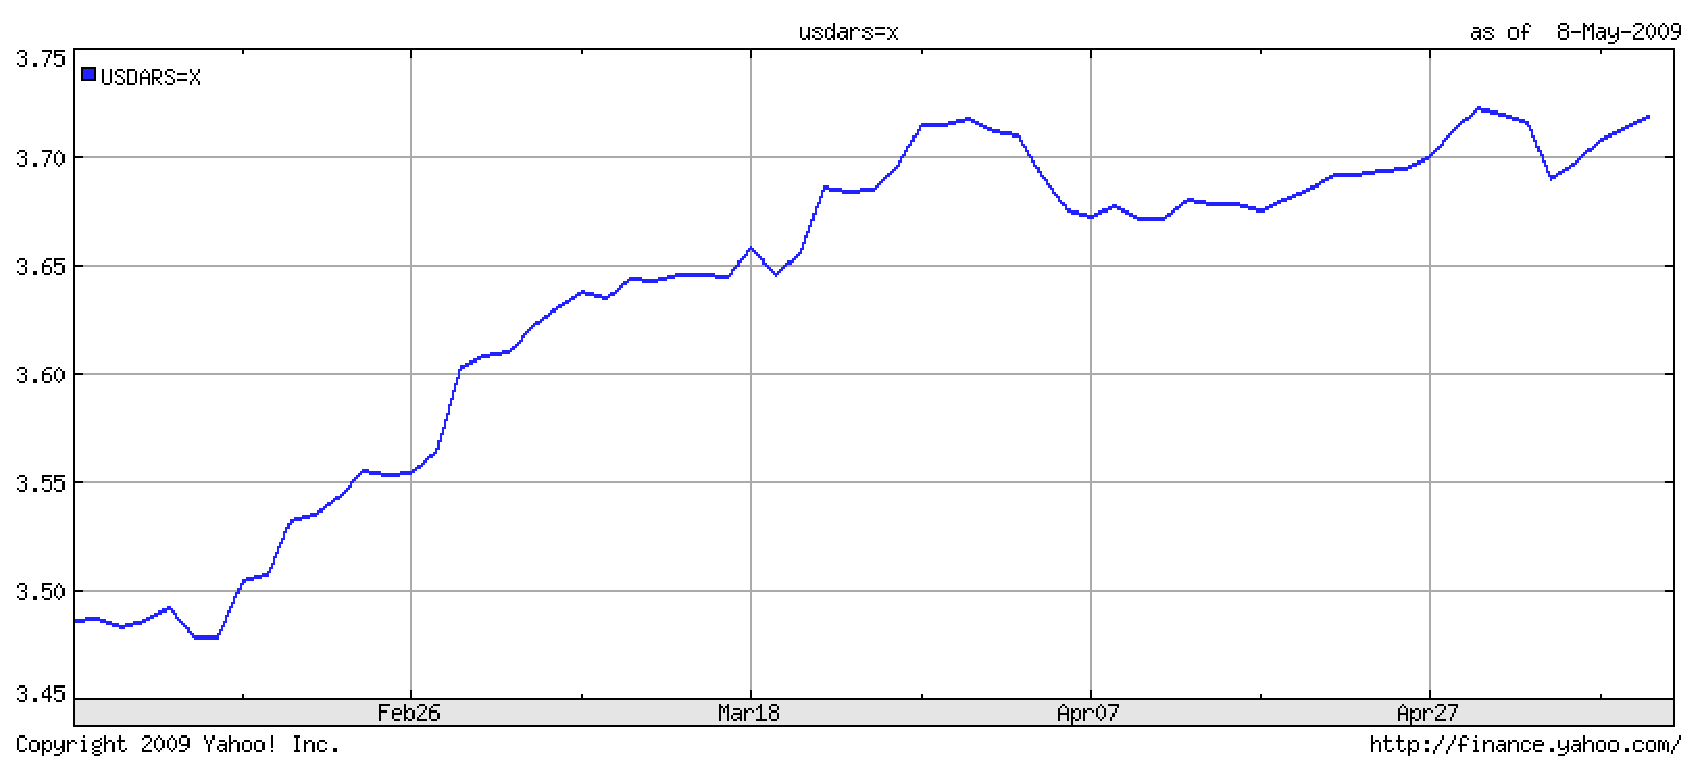
\includegraphics[scale=0.15]{image/usdars.eps}
\end{figure}
+
\begin{figure}
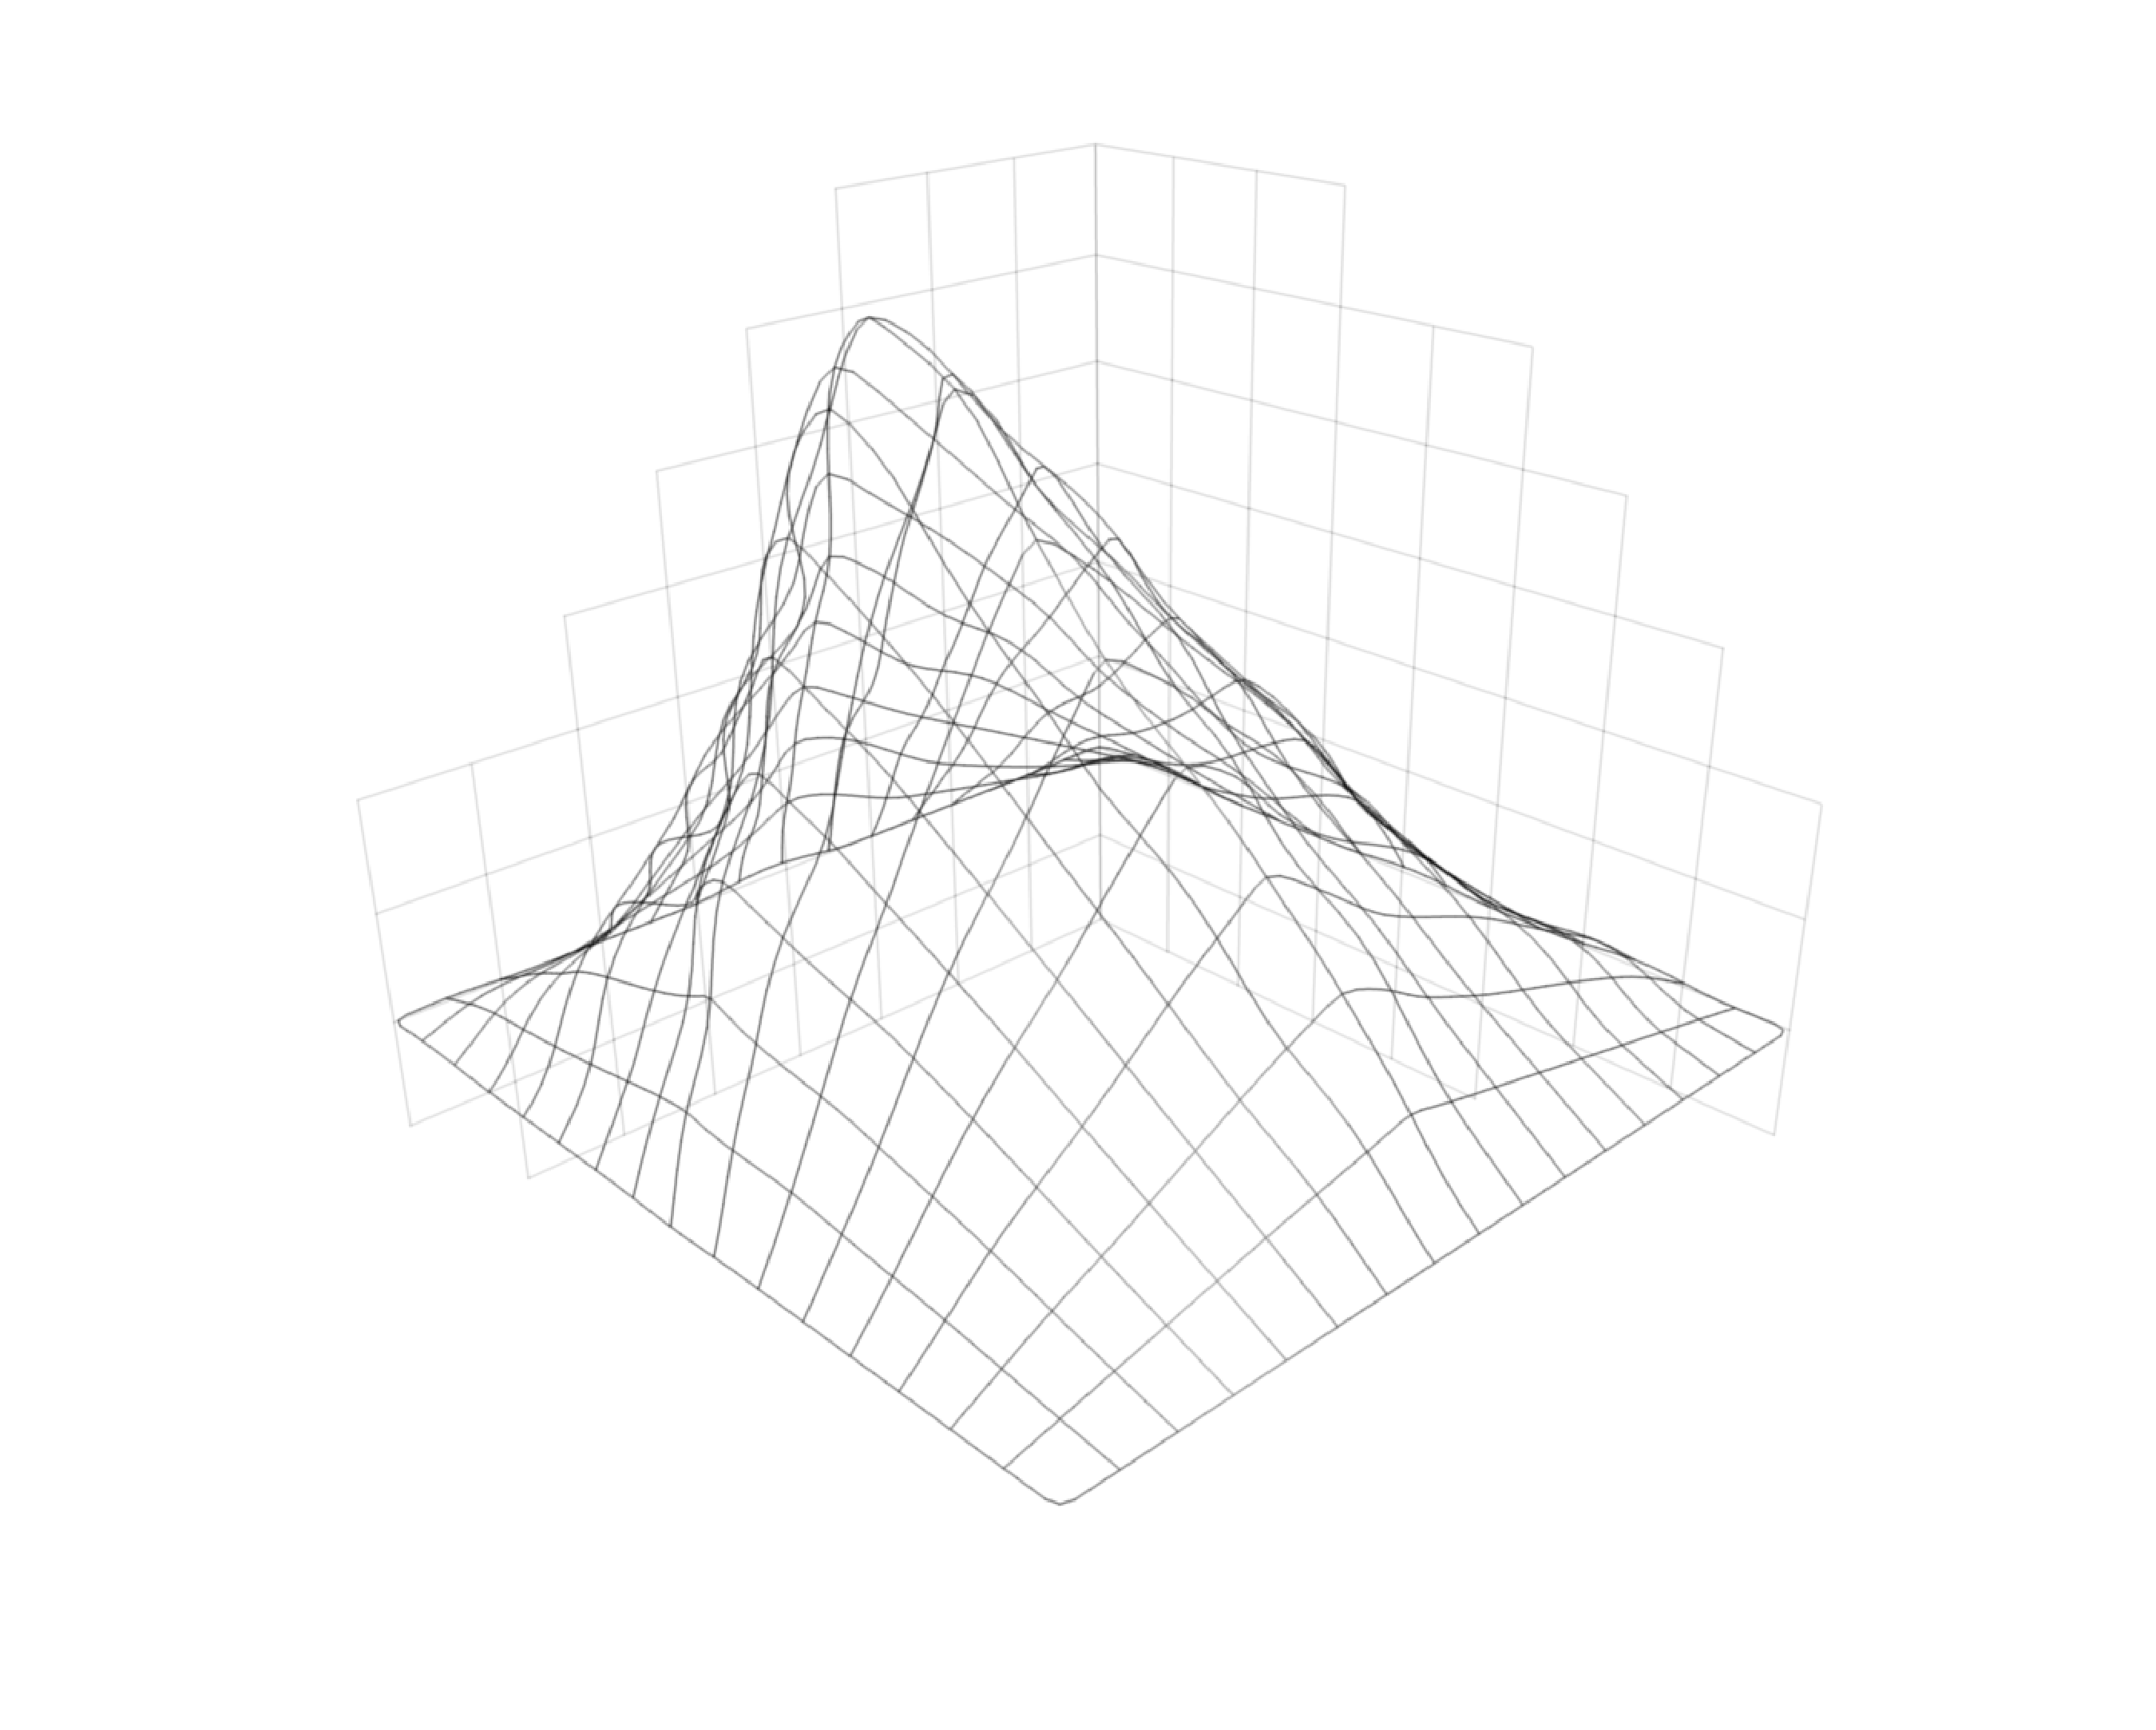
\includegraphics[scale=0.1]{document/image/logo.eps}
\end{figure}
\end{center}
\end{frame}


\subsection{Hipótesis Intrínseca}
\begin{frame}
\frametitle{Hipótesis Intrínseca}
La función aleatoria $Z(u,t)$ es intrínseca en el espacio-tiempo si:
\begin{equation}
E[Z(u,t)] = m
\end{equation}
El \emph{variograma} espacio temporal es independiente de la localización $u$ y del tiempo $t$:
\begin{equation}
\gamma(h,\Delta t) = \frac{1}{2}V[Z(u+h,t+\Delta t) -Z(u,t)]
\end{equation}
\end{frame}

\subsection{Relación entre la distancia y el tiempo}
\begin{frame}
\frametitle{Relación entre la distancia y el tiempo}
\begin{figure}
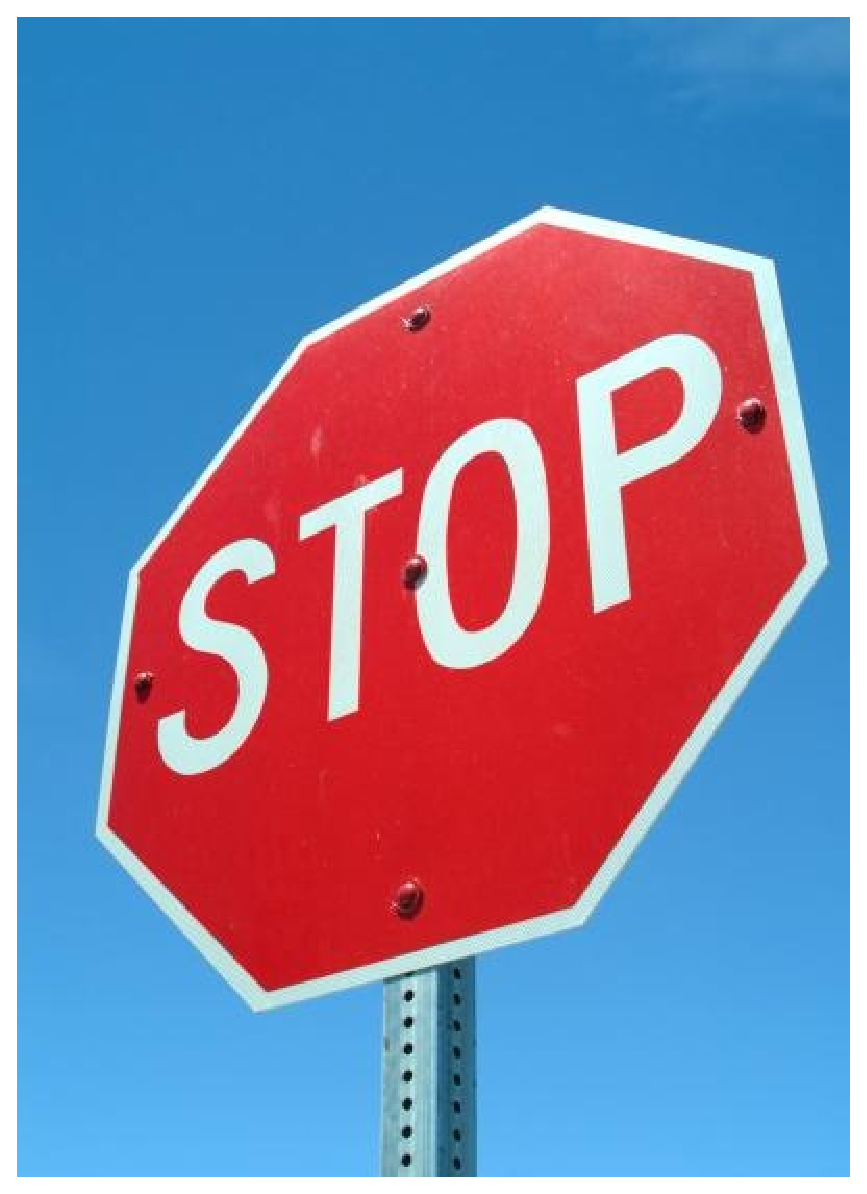
\includegraphics[scale=0.23]{image/stop.eps}
\end{figure}
¿Cuál es el equivalente espacial para una diferencia de tiempo?\\
No hay una función de distancia que relacione al \emph{espacio} y al \emph{tiempo}.
\end{frame}


\subsection{Semivariogramas}
\begin{frame}
\frametitle{Semivariogramas}
Para la componente temporal
\begin{equation}
\gamma_T^*(\Delta t) = \frac{1}{2 N_T(\Delta t)} \sum_{(i,j) \in R_T(\Delta t)} (Z(u_i,t_i)-Z(u_j,t_j))^2
\end{equation}
\begin{description}
\item[$R_T(g)$] $\{ (i,j); g - \varepsilon \leq |t_i - t_j| \leq g + \varepsilon \textit{ y } (u_i = u_j) \}$
\item[$N_T(g)$] Cantidad de elementos en $R_T(g)$.
\end{description}
Para la estructura espacial
\begin{equation}
\gamma_S^*(h) = \frac{1}{2 N_S(h)} \sum_{(i,j) \in R_S(h)} (Z(u_i,t_i)-Z(u_j,t_j))^2
\end{equation}
\begin{description}
\item[$R_S(g)$] $\{ (i,j); g - \varepsilon \leq |u_i - u_j| \leq g + \varepsilon \textit{ y } | t_i - t_j | \leq \delta \}$
\item[$N_S(g)$] Cantidad de elementos en $R_S(g)$.
\end{description}
\end{frame}


\subsection{Relación por anisotropía}
\begin{frame}
\frametitle{Relación por anisotropía}
\begin{itemize}
\item El tipo de los dos variogramas experimentales son similares, tienen el mismo \emph{efecto pepita} y el mismo \emph{tope}. Esto significa que cuanto mucho se observará una \emph{anisotropía geométrica} que será tratada con una transformación lineal, resultando un modelo isotrópico. La \emph{distancia} de un vector $(h,\Delta t)$ se define como:
\begin{equation}
|(h,\Delta t)| = \sqrt{ | h | ^2 + k_t | \Delta t | ^2}
\end{equation}
\item El tipo de los dos variogramas experimentales son diferentes, teniendo una forma diferente y/o un tope distinto. En este caso se modelará un variograma teórico de acuerdo a una \emph{anisotropía zonal}. En este caso el \emph{variograma espacio temporal} $\gamma_{ST}(h,\Delta t)$ puede ser escrito como:
\begin{equation}
\gamma_{ST}(h,\Delta t) = \gamma_S(h) + \gamma_T(\Delta h)
\end{equation}
\end{itemize}
\end{frame}



\section{Referencias}
\begin{frame}
\frametitle{Referencias}
\begin{itemize}
\item Jesús Sánchez Fernández. Introducción a la Estadística Empresarial. 2004. ISBN: 84-688-9882-1.
\item Nguyen Dinh Hoa. The lagrange multiplier function in the equation approach to constrained optimization.
\item András Bárdossy. Introduction to Geostatistics.
\end{itemize}
\end{frame}

\begin{frame}
\frametitle{}
\begin{center}
\huge{¡Muchas Gracias!}
\end{center}
\end{frame}

\end{document}
